\documentclass{ximera}

\author{Anna Davis} \title{MTH 240 Homework 10} 

\begin{document}

\begin{abstract}

\end{abstract}
\maketitle
 \textit{Certificate due: 4/28/2021 at 11:59 p.m.}
 
\begin{problem}\label{prob:240HW10prob1}
Antidifferentiate.
\begin{enumerate}
\item
$\int 6x^2+x^{-2}\,dx=\answer{2x^3-x^{-1}}+C$

\item
$\int \cos x+2e^x\, dx=\answer{\sin x +2e^x}+C$

\item
$\int \frac{x^2+3x-\sqrt{x}}{x}\,dx=\answer{0.5x^2+3x-2\sqrt{x}}+C$

  \end{enumerate}
\end{problem}

\begin{problem}\label{prob:240HW10prob2}
Evaluate the definite integral.

\begin{enumerate}
    \item $\int_1^4 3x^2-2x+3\,dx=\answer{57}$
    \item $\int_0^{\frac{\pi}{2}} \cos x\,dx=\answer{1}$
    \item $\int_{-5}^5 \sqrt{25-x^2}\,dx=\answer[tolerance=0.01]{12.5\pi}$ (enter exact value; no decimal approximations)
\end{enumerate}
\end{problem}

\begin{problem}\label{prob:240HW10prob3}
Find the area under bounded by the graph of $f(x)=4x^3+3x^2-2x+1$ and the $x$-axis on the interval $[-1,1]$.

Area$=\answer{4}$ square units.
\end{problem}


\begin{problem}\label{prob:240HW10prob4}
A graph of $f(x)=x^3-2x^2-11x+12$ is shown below.  Find the total shaded area.  Round your answer to two decimal places.
\begin{image}
   
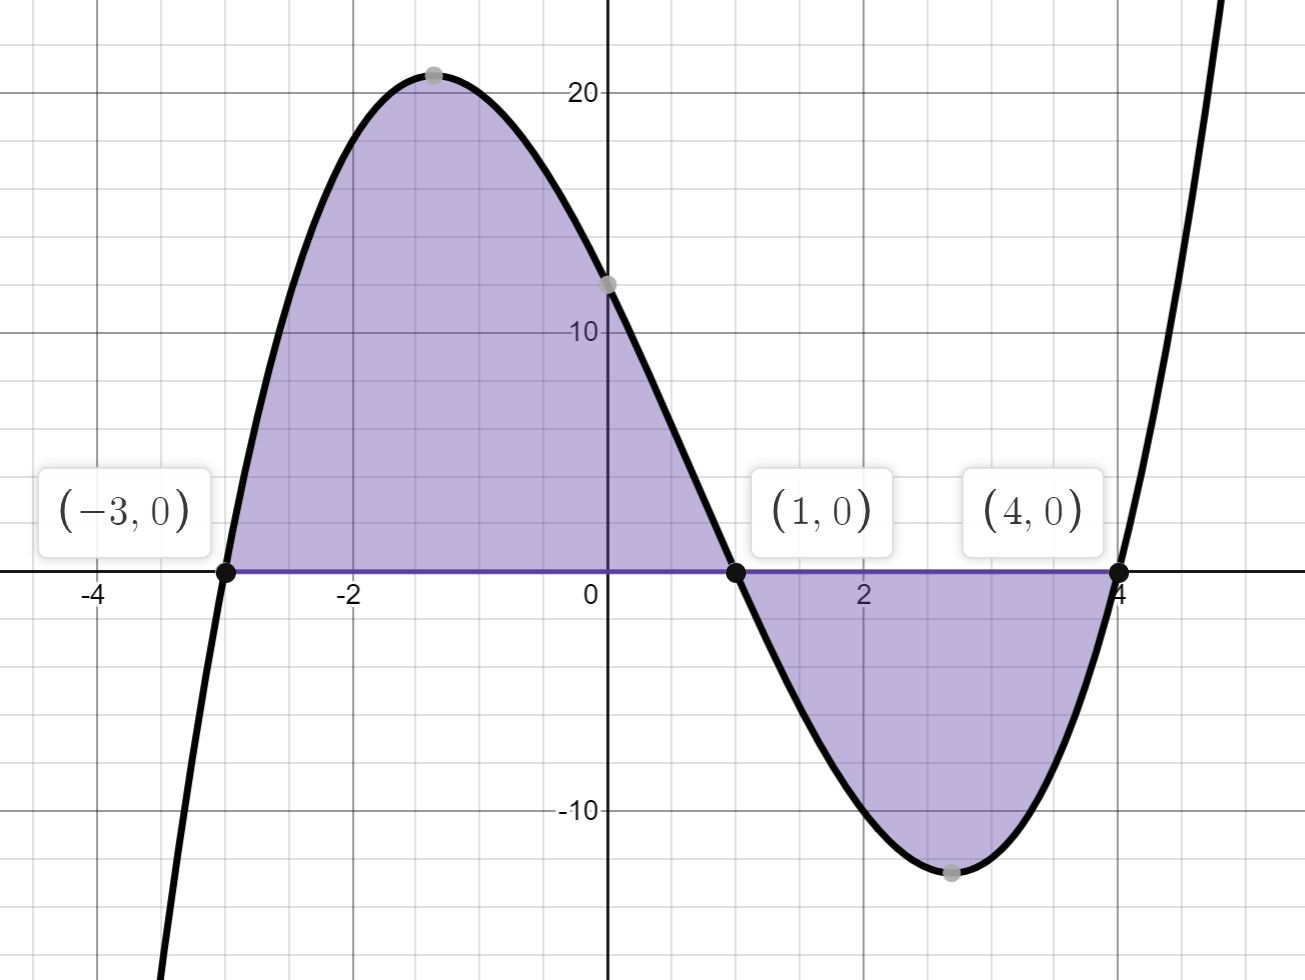
\includegraphics[height=1in]{HW10pic1.jpg}

\end{image}

Total shaded area$=\answer{78.08}$ square units.
\end{problem}


\end{document} 